% Informe final: ¿cuánto va a tardar mi caso? (Anuario Estadístico Judicial 2023 y su serie 2007-2023).
% Compilar desde la carpeta informe/:   pdflatex --disable-installer informe.tex   (dos veces, para el índice)
% Las tablas y las cifras salen de notebooks/22_despliegue.ipynb (carpeta tablas/): no se copian a mano.
\documentclass[11pt,a4paper]{article}

\usepackage[utf8]{inputenc}
\usepackage[T1]{fontenc}
\usepackage{lmodern}
\usepackage[spanish,es-tabla,es-noshorthands]{babel}
\usepackage[margin=2.4cm]{geometry}
\usepackage{microtype}
\usepackage{amsmath}
\usepackage{graphicx}
\usepackage{booktabs}
\usepackage{float}
\usepackage{caption}
\usepackage{xcolor}
\usepackage{tcolorbox}
\usepackage{enumitem}
\usepackage[hidelinks]{hyperref}

\graphicspath{{../web/img/}}
\captionsetup{font=small,labelfont=bf}
\setlist{itemsep=2pt,topsep=4pt}
\definecolor{acento}{HTML}{15604A}
\newtcolorbox{idea}[1][]{colback=acento!6,colframe=acento!70,boxrule=0.6pt,arc=2pt,left=6pt,right=6pt,top=4pt,bottom=4pt,fonttitle=\bfseries\small,#1}

% Generado por notebooks/22_despliegue.ipynb
\newcommand{\nProcesos}{1.240}
\newcommand{\nGrandes}{818}
\newcommand{\nChicos}{422}
\newcommand{\nSinResueltas}{10}
\newcommand{\nFilas}{808}
\newcommand{\nEntrenamiento}{646}
\newcommand{\nPrueba}{162}
\newcommand{\minCausas}{10}
\newcommand{\medianaCausas}{28}
\newcommand{\medianaDias}{221}
\newcommand{\pveinticincoDias}{100}
\newcommand{\psetentaycincoDias}{503}
\newcommand{\nTopados}{13}
\newcommand{\nTiposProceso}{78}
\newcommand{\nOriginales}{19}
\newcommand{\nIngenieria}{8}
\newcommand{\nHistoricas}{1}
\newcommand{\nCompleta}{28}
\newcommand{\nFuga}{19}
\newcommand{\mejorModelo}{Stacking}
\newcommand{\mejorMaeCv}{0,738}
\newcommand{\mejorMaePrueba}{0,694}
\newcommand{\mejorDobPrueba}{67}
\newcommand{\mejorFactorPrueba}{1,52}
\newcommand{\mejorRdosPrueba}{0,41}
\newcommand{\mejorDiasPrueba}{87}
\newcommand{\modeloDesplegado}{Gradient Boosting}
\newcommand{\maeDesplegado}{0,725}
\newcommand{\dobDesplegado}{68}
\newcommand{\factorDesplegado}{1,58}
\newcommand{\rdosDesplegado}{0,38}
\newcommand{\diasDesplegado}{81}
\newcommand{\maeDesplegadoVeintiocho}{0,710}
\newcommand{\coberturaRango}{57}
\newcommand{\nArboles}{100}
\newcommand{\pesoJson}{0,1}
\newcommand{\difJson}{4\times10^{-15}}
\newcommand{\nEntradas}{3}
\newcommand{\histErrVaciado}{11,7}
\newcommand{\histErrVaciadoMedio}{12,4}
\newcommand{\histSesgoVaciado}{5,4}
\newcommand{\histNVaciado}{47}
\newcommand{\histErrAnterior}{8,8}
\newcommand{\histPeorAnterior}{35}
\newcommand{\histErrIngenua}{25,0}
\newcommand{\histSesgoIngenua}{-24,1}
\newcommand{\histErrRitmo}{18,2}
\newcommand{\histTiempoDosmilsiete}{359}
\newcommand{\histTiempoDosmildoce}{448}
\newcommand{\histTiempoDosmilquince}{316}
\newcommand{\histTiempoDosmilveinte}{485}
\newcommand{\histTiempoDosmilveintitres}{340}
\newcommand{\histCapitalDosmilveintitres}{331}
\newcommand{\histProvinciaDosmilveintitres}{365}
\newcommand{\topVarA}{log del stock heredado}
\newcommand{\topVarB}{presión del stock}
\newcommand{\topVarC}{log de los ingresos}
\newcommand{\topVarD}{ingresos por juzgado}
\newcommand{\topVarE}{stock por juzgado}
\newcommand{\maeDefBase}{1,085}
\newcommand{\maeCvBase}{1,085}
\newcommand{\maePruebaBase}{1,078}
\newcommand{\dobPruebaBase}{42}
\newcommand{\rdosPruebaBase}{-0,00}
\newcommand{\maeDefIngenua}{0,888}
\newcommand{\maeCvIngenua}{0,888}
\newcommand{\maePruebaIngenua}{0,858}
\newcommand{\dobPruebaIngenua}{65}
\newcommand{\rdosPruebaIngenua}{0,11}
\newcommand{\maeDefRidge}{0,796}
\newcommand{\maeCvRidge}{0,787}
\newcommand{\maePruebaRidge}{0,718}
\newcommand{\dobPruebaRidge}{64}
\newcommand{\rdosPruebaRidge}{0,50}
\newcommand{\maeVDiecinueveCvRidge}{0,921}
\newcommand{\maeVDiecinuevePruebaRidge}{0,943}
\newcommand{\maeVVeintiochoCvRidge}{0,787}
\newcommand{\maeVVeintiochoPruebaRidge}{0,718}
\newcommand{\maeVCincoCvRidge}{0,800}
\newcommand{\maeVCincoPruebaRidge}{0,695}
\newcommand{\maeDefSVM}{0,790}
\newcommand{\maeCvSVM}{0,751}
\newcommand{\maePruebaSVM}{0,697}
\newcommand{\dobPruebaSVM}{65}
\newcommand{\rdosPruebaSVM}{0,41}
\newcommand{\maeVDiecinueveCvSVM}{0,850}
\newcommand{\maeVDiecinuevePruebaSVM}{0,844}
\newcommand{\maeVVeintiochoCvSVM}{0,751}
\newcommand{\maeVVeintiochoPruebaSVM}{0,697}
\newcommand{\maeVCincoCvSVM}{0,773}
\newcommand{\maeVCincoPruebaSVM}{0,718}
\newcommand{\maeDefBagging}{0,804}
\newcommand{\maeCvBagging}{0,752}
\newcommand{\maePruebaBagging}{0,731}
\newcommand{\dobPruebaBagging}{68}
\newcommand{\rdosPruebaBagging}{0,39}
\newcommand{\maeVDiecinueveCvBagging}{0,815}
\newcommand{\maeVDiecinuevePruebaBagging}{0,821}
\newcommand{\maeVVeintiochoCvBagging}{0,752}
\newcommand{\maeVVeintiochoPruebaBagging}{0,731}
\newcommand{\maeVCincoCvBagging}{0,820}
\newcommand{\maeVCincoPruebaBagging}{0,756}
\newcommand{\maeDefRandomForest}{0,767}
\newcommand{\maeCvRandomForest}{0,752}
\newcommand{\maePruebaRandomForest}{0,736}
\newcommand{\dobPruebaRandomForest}{64}
\newcommand{\rdosPruebaRandomForest}{0,35}
\newcommand{\maeVDiecinueveCvRandomForest}{0,830}
\newcommand{\maeVDiecinuevePruebaRandomForest}{0,828}
\newcommand{\maeVVeintiochoCvRandomForest}{0,752}
\newcommand{\maeVVeintiochoPruebaRandomForest}{0,736}
\newcommand{\maeVCincoCvRandomForest}{0,807}
\newcommand{\maeVCincoPruebaRandomForest}{0,753}
\newcommand{\maeDefAdaBoost}{0,890}
\newcommand{\maeCvAdaBoost}{0,755}
\newcommand{\maePruebaAdaBoost}{0,772}
\newcommand{\dobPruebaAdaBoost}{67}
\newcommand{\rdosPruebaAdaBoost}{0,30}
\newcommand{\maeVDiecinueveCvAdaBoost}{0,862}
\newcommand{\maeVDiecinuevePruebaAdaBoost}{0,900}
\newcommand{\maeVVeintiochoCvAdaBoost}{0,755}
\newcommand{\maeVVeintiochoPruebaAdaBoost}{0,772}
\newcommand{\maeVCincoCvAdaBoost}{0,814}
\newcommand{\maeVCincoPruebaAdaBoost}{0,767}
\newcommand{\maeDefGradientBoosting}{0,780}
\newcommand{\maeCvGradientBoosting}{0,746}
\newcommand{\maePruebaGradientBoosting}{0,710}
\newcommand{\dobPruebaGradientBoosting}{68}
\newcommand{\rdosPruebaGradientBoosting}{0,39}
\newcommand{\maeVDiecinueveCvGradientBoosting}{0,809}
\newcommand{\maeVDiecinuevePruebaGradientBoosting}{0,777}
\newcommand{\maeVVeintiochoCvGradientBoosting}{0,746}
\newcommand{\maeVVeintiochoPruebaGradientBoosting}{0,710}
\newcommand{\maeVCincoCvGradientBoosting}{0,794}
\newcommand{\maeVCincoPruebaGradientBoosting}{0,725}
\newcommand{\maeDefStacking}{0,751}
\newcommand{\maeCvStacking}{0,738}
\newcommand{\maePruebaStacking}{0,694}
\newcommand{\dobPruebaStacking}{67}
\newcommand{\rdosPruebaStacking}{0,41}
\newcommand{\maeVDiecinueveCvStacking}{0,796}
\newcommand{\maeVDiecinuevePruebaStacking}{0,770}
\newcommand{\maeVVeintiochoCvStacking}{0,738}
\newcommand{\maeVVeintiochoPruebaStacking}{0,694}
\newcommand{\maeVCincoCvStacking}{0,770}
\newcommand{\maeVCincoPruebaStacking}{0,716}
\newcommand{\maeGruposDiecinueveStacking}{0,810}
\newcommand{\difGruposDiecinueveStacking}{0,014}
\newcommand{\maeGruposDiecinueveRandomForest}{0,822}
\newcommand{\difGruposDiecinueveRandomForest}{-0,008}
\newcommand{\maeGruposDiecinueveSVM}{0,875}
\newcommand{\difGruposDiecinueveSVM}{0,025}
\newcommand{\maeGruposVeintiochoStacking}{0,764}
\newcommand{\difGruposVeintiochoStacking}{0,026}
\newcommand{\maeGruposVeintiochoRandomForest}{0,766}
\newcommand{\difGruposVeintiochoRandomForest}{0,014}
\newcommand{\maeGruposVeintiochoSVM}{0,812}
\newcommand{\difGruposVeintiochoSVM}{0,061}
\newcommand{\maeGruposCincoStacking}{0,778}
\newcommand{\difGruposCincoStacking}{0,007}
\newcommand{\maeGruposCincoRandomForest}{0,831}
\newcommand{\difGruposCincoRandomForest}{0,024}
\newcommand{\maeGruposCincoSVM}{0,771}
\newcommand{\difGruposCincoSVM}{-0,002}
\newcommand{\dobTamanoA}{47}
\newcommand{\dobTamanoB}{62}
\newcommand{\dobTamanoC}{78}
\newcommand{\dobTamanoD}{88}
\newcommand{\impHistorica}{0,0050}
\newcommand{\rangoHistorica}{17}
\newcommand{\svmC}{10}
\newcommand{\svmGamma}{0,010}
\newcommand{\svmEpsilon}{0,1}
\newcommand{\maeSvmMin}{0,751}
\newcommand{\maeSvmMax}{1,025}
\newcommand{\rhoPresion}{0,64}
\newcommand{\rhoIngresos}{-0,20}
\newcommand{\rhoStock}{0,23}
\newcommand{\rhoHistorica}{0,16}
\newcommand{\rangoChicoDesde}{0,43}
\newcommand{\rangoChicoHasta}{2,35}
\newcommand{\rangoGrandeDesde}{0,66}
\newcommand{\rangoGrandeHasta}{1,44}


\hypersetup{pdftitle={¿Cuánto va a tardar mi caso?},
  pdfauthor={Andrés Maximiliano Espinoza Romero, Andrés Gabriel Maydana García, Maximiliano Gómez Mallo}}

\begin{document}

%--------------------------------------------------------------------- portada
\begin{titlepage}
  \centering
  {\Large\bfseries\color{acento!40!black} UNIVERSIDAD MAYOR DE SAN ANDRÉS\par}
  \vspace{1.2cm}
  
\includegraphics[height=7.2cm]{img/umsa.png}\par
  \vspace{1.3cm}
  {\color{acento}\rule{0.75\linewidth}{1.2pt}\par}
  \vspace{0.5cm}
  {\LARGE\bfseries ¿Cuánto va a tardar mi caso?\par}
  \vspace{0.35cm}
  {\large Estimación del tiempo de los procesos judiciales con el Anuario Estadístico Judicial\\
   y su historia 2007--2023: preprocesamiento, modelos de regresión, evaluación y despliegue\par}
  \vspace{0.5cm}
  {\color{acento}\rule{0.75\linewidth}{1.2pt}\par}
  \vfill
  \begin{tabular}{@{}r@{\hspace{0.8em}}l@{}}
    \textbf{Materia:} & Análisis de Datos \\[3pt]
    \textbf{Docente:} & M.Sc. Madelina Loza Soliz \\[3pt]
    \textbf{Integrantes:} & Andrés Maximiliano Espinoza Romero \\
                          & Andrés Gabriel Maydana García \\
                          & Maximiliano Gómez Mallo \\
  \end{tabular}
  \vfill
  {\large La Paz -- Bolivia\par}
  {\large Noviembre de 2026\par}
\end{titlepage}

\begin{abstract}
\noindent
Quien presenta un divorcio, una demanda laboral o un cobro quiere saber una cosa: \emph{¿cuánto va a tardar?} El
Anuario Estadístico Judicial de Bolivia no sigue causas una por una, pero publica para cada tipo de proceso y cada lugar
cuántas causas había, cuántas entraron y cuántas se resolvieron, y trae además el movimiento de causas del país desde
2007. Con eso se mide el tiempo de la \emph{fila}: causas pendientes al cierre entre causas resueltas en el año, en días.
Este informe usa la \textbf{historia 2007--2023} para comprobar que esa medida funciona ---el tiempo estimado quedó a una
mediana de \histErrVaciado~\% de lo que la fila de verdad tardó en vaciarse en \histNVaciado{} comprobaciones, y de un año
al siguiente cambia una mediana de \histErrAnterior~\%--- y entrena modelos de \textbf{regresión} que estiman ese tiempo
con lo que se sabe al presentar el caso: la fila que espera, las causas que entran, los juzgados, la materia, el lugar y
la tendencia histórica de la materia. Siguiendo el orden pedido se presentan (1)~el preprocesamiento, (2)~los modelos
---SVM, Bagging, Boosting y Stacking--- con ajuste de hiperparámetros, (3)~la evaluación, con la importancia de las
variables y la comparación entre las \nOriginales{} originales, las \nCompleta{} con ingeniería e historia y las 5 más
importantes, y (4)~el despliegue del modelo de 5~variables en una página pública. Con \nFilas{} procesos no penales de
2023, el mejor modelo (\mejorModelo) deja al \mejorDobPrueba~\% de los procesos de prueba entre la mitad y el doble de su
tiempo real (88~\% en los procesos grandes); el modelo publicado (\modeloDesplegado, 5 variables que salen de solo 3
datos) logra \dobDesplegado~\% y acompaña cada estimación con un rango probable.
\end{abstract}

\tableofcontents
\newpage

%=====================================================================
\section*{Introducción}
\addcontentsline{toc}{section}{Introducción}

\paragraph{El problema práctico.} En Bolivia una persona que inicia un proceso judicial no tiene ninguna forma pública
de saber cuánto va a esperar. La respuesta habitual es «depende», y es cierto: depende del juzgado, de las partes, de las
pruebas. Pero también depende de algo que sí se puede medir: \emph{cuántas causas tiene delante} y \emph{a qué ritmo las
resuelven los juzgados} de su materia en su ciudad. El objetivo de este informe es estimar ese tiempo para cada tipo de
proceso y lugar, con un rango honesto, y ponerlo al alcance de cualquiera en una página web.

\paragraph{La medida: el tiempo de la fila.} El Anuario publica, para cada tipo de proceso de cada capital y provincia,
el stock con el que empezó el año, las causas que ingresaron, las resueltas y las pendientes al cierre. Con eso:
\begin{equation*}
  \text{tiempo estimado (días)} = \frac{\text{causas pendientes al cierre}}{\text{causas resueltas en el año}}\times 365 .
\end{equation*}
Si quedan 600 causas esperando y el juzgado resuelve 1.200 al año, la fila se termina en medio año; un caso nuevo se pone
al final de esa fila. Es la «duración estimada» que usa el Centro de Estudios de Justicia de las Américas (CEJA) y que el
notebook~10 del proyecto ya calculaba. Es un número de días, así que el problema es de \textbf{regresión}.

\paragraph{La historia.} Un solo año no alcanza para saber si la medida sirve. Por eso se usa el capítulo~9 del Anuario,
que trae el movimiento de causas del país, de las capitales y de las provincias de 2007 a 2023, y las causas resueltas por
materia de 2020 a 2023. Con esos años se responde lo que 2023 solo no puede: si el tiempo estimado se parece a lo que la
fila \emph{de verdad} tardó en vaciarse, y cuánto cambia de un año al siguiente.

\paragraph{Los datos del modelo.} Cada fila es un tipo de proceso en un territorio y una materia (por ejemplo,
«divorcio, familia, Sucre capital»). Se usan las cinco materias no penales (civil y comercial, familia, niñez y
adolescencia, trabajo, coactivo fiscal), porque las penales no publican causas resueltas. De los \nProcesos{} procesos no
penales con movimiento en 2023 entran al modelo los \nFilas{} con al menos \minCausas{} causas atendidas y alguna resuelta,
de \nTiposProceso{} tipos de proceso distintos. Todo el código está en notebooks ejecutados: del \texttt{01} al
\texttt{18}, la construcción y el análisis exploratorio de los datos; del \texttt{19} al \texttt{23}, lo que presenta
este informe.

%=====================================================================
\section{Preprocesamiento}

\subsection{De dónde vienen los datos}
El PDF de 774 páginas no tiene datos abiertos. Los notebooks 01 a 07 lo inventariaron página por página y extrajeron sus
cuadros con técnicas distintas según el formato (por posición, por coordenadas y por firmas de encabezado). Los notebooks
04 a 06 normalizaron materias, territorios y números con la convención boliviana (punto de miles, coma decimal) y
exportaron doce tablas con 85.953 filas, cada una con su cuadro y su página de origen. El notebook 05 verificó doce
identidades contables del propio Anuario y registró 117 discrepancias de la fuente, sin corregirlas. El 08 integró las
tablas en una capa analítica, y los notebooks 09 a 18 hicieron el análisis exploratorio: indicadores de congestión,
valores atípicos, la serie 2007--2023, la concentración del rezago y los recursos de cada departamento.

\subsection{Lo que enseña la historia (2007--2023)}

\paragraph{El tiempo, año por año.} Con los cuadros 9.1.4, 9.1.8 y 9.1.12 (todas las materias, penales incluidas) se
calculó el tiempo estimado de cada año. El país pasó de \histTiempoDosmilsiete{} días en 2007 a \histTiempoDosmildoce{} en
2012, bajó a \histTiempoDosmilquince{} en 2015, saltó a \histTiempoDosmilveinte{} en la pandemia y quedó en
\histTiempoDosmilveintitres{} en 2023, el valor más bajo desde 2015. En 2023 las capitales (\histCapitalDosmilveintitres{}
días) ya son más rápidas que las provincias (\histProvinciaDosmilveintitres) (figura~\ref{fig:historia}, izquierda).

\paragraph{¿La fila se vació en el tiempo estimado?} Al cierre de cada año quedan $P$ causas pendientes y el tiempo
estimado dice que se terminarán en $P/R\times365$ días. Con los años siguientes se puede ver cuánto tardó \emph{de
verdad} el sistema en resolver esa cantidad de causas: se suman las resueltas de los años siguientes hasta llegar a $P$
(dentro del último año, en proporción a los días). En \histNVaciado{} comprobaciones (país, capitales y provincias,
2007--2022) la diferencia mediana fue de \textbf{\histErrVaciado~\%} (media \histErrVaciadoMedio~\%), con un leve sesgo
pesimista: el tiempo estimado tiende a pasarse en \histSesgoVaciado~\% (tabla~\ref{tab:vaciado}). Es una comprobación
aproximada, porque supone que las causas se resuelven en orden de llegada y el Anuario no dice cuáles se resolvieron,
solo cuántas; aun así, muestra que la medida \emph{mide lo que dice medir}.

\begin{table}[H]
  \centering\small
  \caption{El país: tiempo estimado al cierre de cada año y lo que la fila de verdad tardó en vaciarse con las
  resoluciones de los años siguientes. Notebook 19.}
  \label{tab:vaciado}
  \begin{tabular}{rrrr}
\toprule
Año & Tiempo estimado (días) & Lo que de verdad tardó (días) & Diferencia \\
\midrule
2007 & 359 & 313 & +15\,\% \\
2008 & 355 & 338 & +5\,\% \\
2009 & 392 & 384 & +2\,\% \\
2010 & 427 & 414 & +3\,\% \\
2011 & 445 & 380 & +17\,\% \\
2012 & 448 & 388 & +15\,\% \\
2013 & 417 & 398 & +5\,\% \\
2014 & 404 & 328 & +23\,\% \\
2015 & 316 & 357 & -11\,\% \\
2016 & 393 & 466 & -16\,\% \\
2017 & 384 & 394 & -2\,\% \\
2018 & 352 & 363 & -3\,\% \\
2019 & 388 & 470 & -18\,\% \\
2020 & 485 & 380 & +28\,\% \\
2021 & 377 & 358 & +5\,\% \\
2022 & 379 & 348 & +9\,\% \\
\bottomrule
\end{tabular}

\end{table}

\paragraph{¿Cuánto cambia de un año al siguiente?} Si el tiempo de este año se parece al del próximo, el último Anuario
sirve para quien presenta su caso después. Se compararon tres formas de anticipar el tiempo de un año con lo que se sabía
antes (tabla~\ref{tab:formas}). Usar \textbf{el tiempo del año anterior} se equivoca en una mediana de
\histErrAnterior~\% (el peor caso, \histPeorAnterior~\%, en la pandemia). La \textbf{fórmula ingenua} ---stock heredado
entre ingresos, que supone que se resuelve todo lo que entra--- se equivoca \histErrIngenua~\% y siempre se queda corta
(sesgo \histSesgoIngenua~\%). Por eso la fórmula ingenua es una de las referencias que el modelo debe superar.

\begin{table}[H]
  \centering\small
  \caption{Tres formas de anticipar el tiempo de un año, comprobadas con la serie 2007--2023 (país, capitales y
  provincias). Error porcentual respecto del tiempo real del año. Notebook 19.}
  \label{tab:formas}
  \resizebox{\linewidth}{!}{\begin{tabular}{lrrrr}
\toprule
Forma de anticipar el tiempo del año & Error mediano & Error medio & Sesgo & Peor año \\
\midrule
el del año anterior & 8,8\,\% & 10,3\,\% & -0,4\,\% & 35,2\,\% \\
fórmula ingenua & 25,0\,\% & 24,7\,\% & -24,1\,\% & 51,1\,\% \\
stock ÷ ritmo anterior & 18,2\,\% & 15,3\,\% & -10,6\,\% & 40,7\,\% \\
\bottomrule
\end{tabular}
}
\end{table}

\paragraph{Las materias.} Por materia el Anuario solo trae las \emph{resueltas} de 2019 a 2023 (cuadros 9.1.2 y 9.1.6).
2019 no se usa porque no cuadra con los totales (notebook 15) y 2020 es el año de la pandemia. De 2020 a 2023 las
resoluciones crecieron en todas las materias no penales (figura~\ref{fig:historia}, derecha). De ahí sale la
\textbf{variable histórica} del modelo: cuánto cambiaron las resoluciones de la materia, en su ámbito, \emph{el año
anterior} al caso. Para un caso de 2023 es $\text{resueltas}_{2022}/\text{resueltas}_{2021}-1$; para uno de 2024,
$\text{resueltas}_{2023}/\text{resueltas}_{2022}-1$. Usa solo años pasados, así que no espía el año que se predice.

\begin{figure}[H]
  \centering
  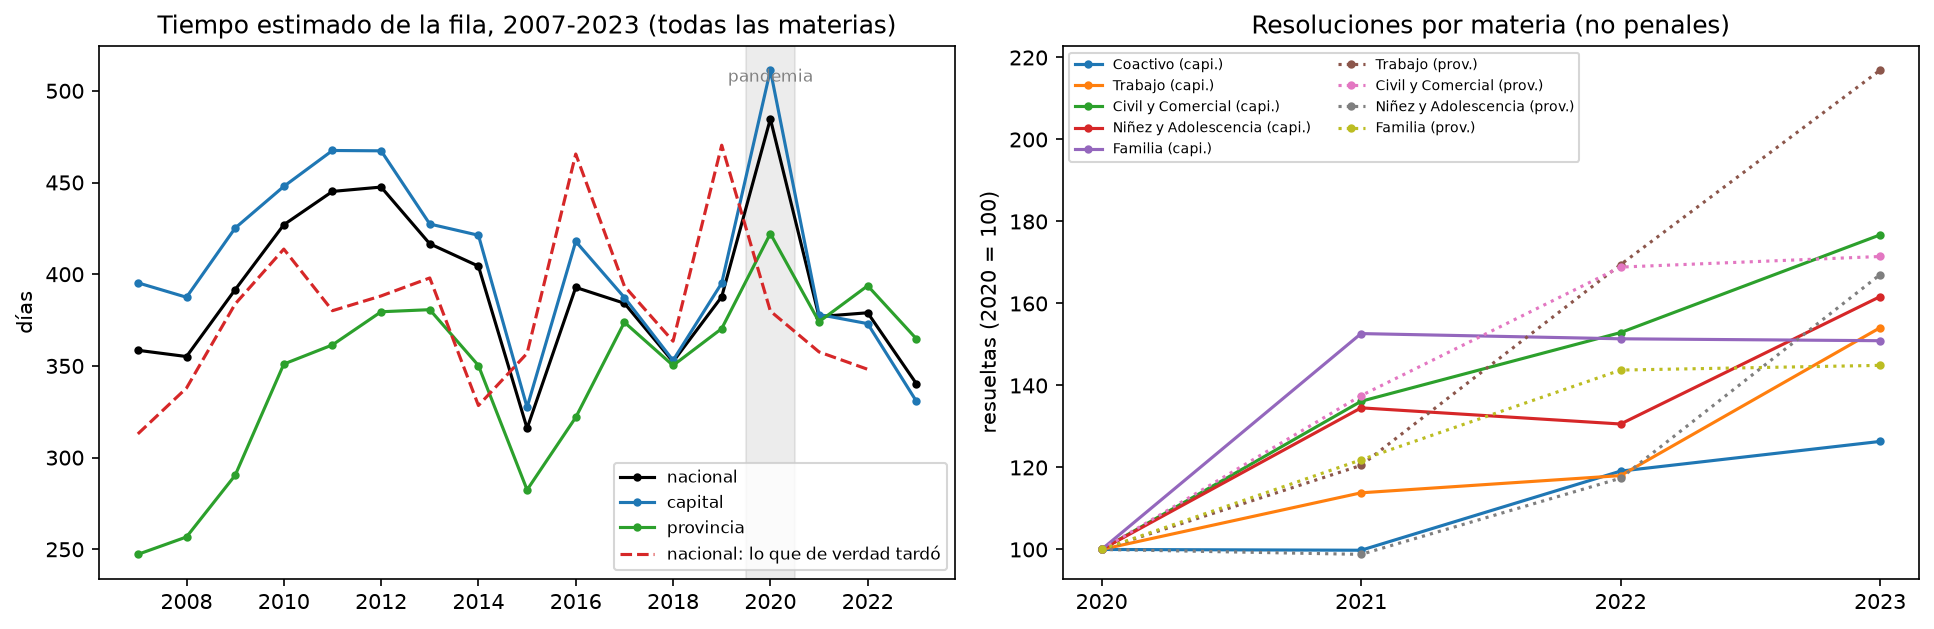
\includegraphics[width=\linewidth]{nb19_1.png}
  \caption{Izquierda: tiempo estimado de la fila en el país, las capitales y las provincias, 2007--2023, y lo que la fila
  del país de verdad tardó en vaciarse (línea roja). Derecha: causas resueltas por materia no penal, con 2020~$=$~100.
  Notebook 19.}
  \label{fig:historia}
\end{figure}

\subsection{Análisis exploratorio del objetivo}
El tiempo mediano de los \nFilas{} procesos es de \medianaDias{} días; la mitad está entre \pveinticincoDias{} y
\psetentaycincoDias. Las materias difieren mucho (mediana: coactivo fiscal 887 días, trabajo 375, civil 243, familia 195,
niñez 146); capital y provincia, poco (209 contra 236). La variable que más acompaña al tiempo es la \textbf{presión del
stock}, el stock heredado entre los ingresos ($\rho=\rhoPresion$ de Spearman): donde la fila heredada es grande en relación
con lo que entra, se tarda más. Los ingresos van al revés ($\rho=\rhoIngresos$): los procesos con mucho movimiento
resuelven rápido. La variable histórica tiene una relación débil ($\rho=\rhoHistorica$). El tiempo tiene una cola larga a
la derecha; en logaritmo se vuelve manejable (figura~\ref{fig:eda}).

\begin{figure}[H]
  \centering
  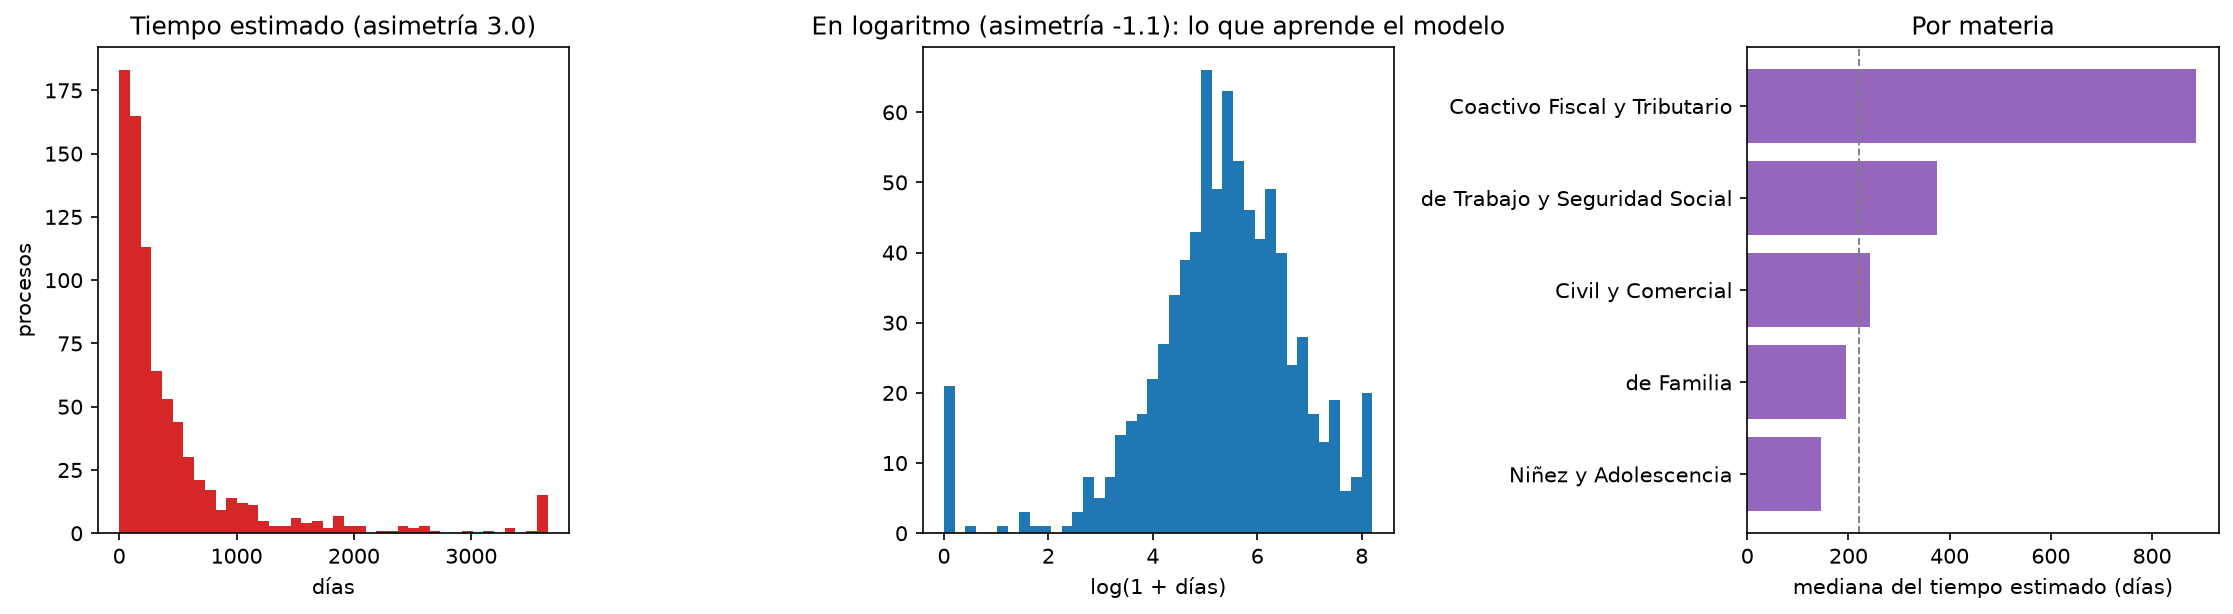
\includegraphics[width=\linewidth]{nb19_2.png}
  \caption{El tiempo estimado en días (cola larga), en $\log(1+\text{días})$ (lo que aprende el modelo) y su mediana por
  materia. Notebook 19.}
  \label{fig:eda}
\end{figure}

\subsection{Limpieza}

\paragraph{Qué filas entran.} De los \nProcesos{} procesos con movimiento se dejan fuera los \nChicos{} con menos de
\minCausas{} causas atendidas: en la mitad de los procesos hubo \medianaCausas{} causas o menos en todo el año, y con una
resuelta y dos pendientes el «tiempo» sería 730 días; con una resuelta más, 243. Eso no mide una fila, mide la suerte de
una causa. El filtro usa las causas \emph{atendidas} (stock heredado más ingresos: un dato de entrada), no las resueltas ni
el tiempo, así que no elige ejemplos mirando la respuesta. También quedan fuera los \nSinResueltas{} procesos con 10 o más
causas y ninguna resuelta, porque su tiempo no existe (dividir por cero). La página pública muestra igual unos y otros,
con una advertencia.

\paragraph{Fuga de información.} Es el error más grave al preparar un modelo: usar como pista algo que contiene la
respuesta. El tiempo se calcula con las resueltas y los pendientes al cierre; toda columna hecha con ellos le dice al
modelo la respuesta. Se excluyeron \nFuga{} columnas (tabla~\ref{tab:fuga}); el notebook 19 comprueba con un
\texttt{assert} que ninguna entra al modelo.

\begin{table}[H]
  \centering\small
  \caption{Columnas excluidas por fuga de información.}
  \label{tab:fuga}
  \begin{tabular}{lp{9cm}}
\toprule
Columna excluida & Motivo \\
\midrule
\texttt{resueltas} & es parte de la respuesta: el tiempo se divide por las resueltas \\
\texttt{pendientes\_fin} & es parte de la respuesta: el tiempo es pendientes al cierre / resueltas \\
\texttt{duracion\_estimada\_dias} & es el objetivo \\
\texttt{duracion\_estimada\_winsorizada} & es el objetivo recortado \\
\texttt{tasa\_resolucion} & resueltas / ingresos \\
\texttt{tasa\_resolucion\_con\_readecuadas} & usa resueltas \\
\texttt{tasa\_resolucion\_solo\_nuevas} & usa resueltas \\
\texttt{tasa\_congestion} & atendidas / resueltas \\
\texttt{tasa\_pendencia} & usa pendientes al cierre \\
\texttt{acumulacion\_neta\_anual} & ingresos - resueltas \\
\texttt{flag\_acumula\_mora} & usa resueltas \\
\texttt{flag\_sin\_resolucion\_anual} & usa resueltas \\
\texttt{flag\_sin\_movimiento} & usa resueltas \\
\texttt{estado\_gestion} & clasifica la fila según sus resueltas \\
\texttt{tasa\_congestion\_winsorizada} & usa resueltas \\
\texttt{log\_resueltas} & usa resueltas \\
\texttt{log\_pendientes\_fin} & usa pendientes al cierre \\
\texttt{es\_outlier\_congestion\_iqr} & marca construida con la tasa de congestión \\
\texttt{es\_outlier\_duracion\_iqr} & marca construida con el tiempo \\
\bottomrule
\end{tabular}

\end{table}

\paragraph{Valores faltantes.} Casi todos los vacíos son \emph{estructurales}: la columna no existe para esa materia. Dos
formas de ingreso (preliminares y cautelares formalizados) solo existen en civil; en las otras materias el vacío es un
cero y se llenó con 0. Imputarlas con la mediana inventaría causas que no existen. El único faltante real es el número de
tribunales del territorio (4 filas): se imputa con la mediana \emph{del entrenamiento}, dentro del modelo, para que la
prueba no influya en el valor imputado.

\paragraph{Valores atípicos.} No se eliminan procesos: uno con miles de causas es real (el notebook 11 lo comprobó contra
el PDF). Dos decisiones: el objetivo se \textbf{recorta en 10 años} (\nTopados{} procesos pasan de ese tope; más que eso
es «no se mueve», y un número como 80 años no es un plazo), y se modela su \textbf{logaritmo}, que acerca los extremos sin
borrarlos. Para los modelos sensibles a la escala se agregan versiones en logaritmo y cocientes de las cantidades
(figura~\ref{fig:asimetria}).

\begin{figure}[H]
  \centering
  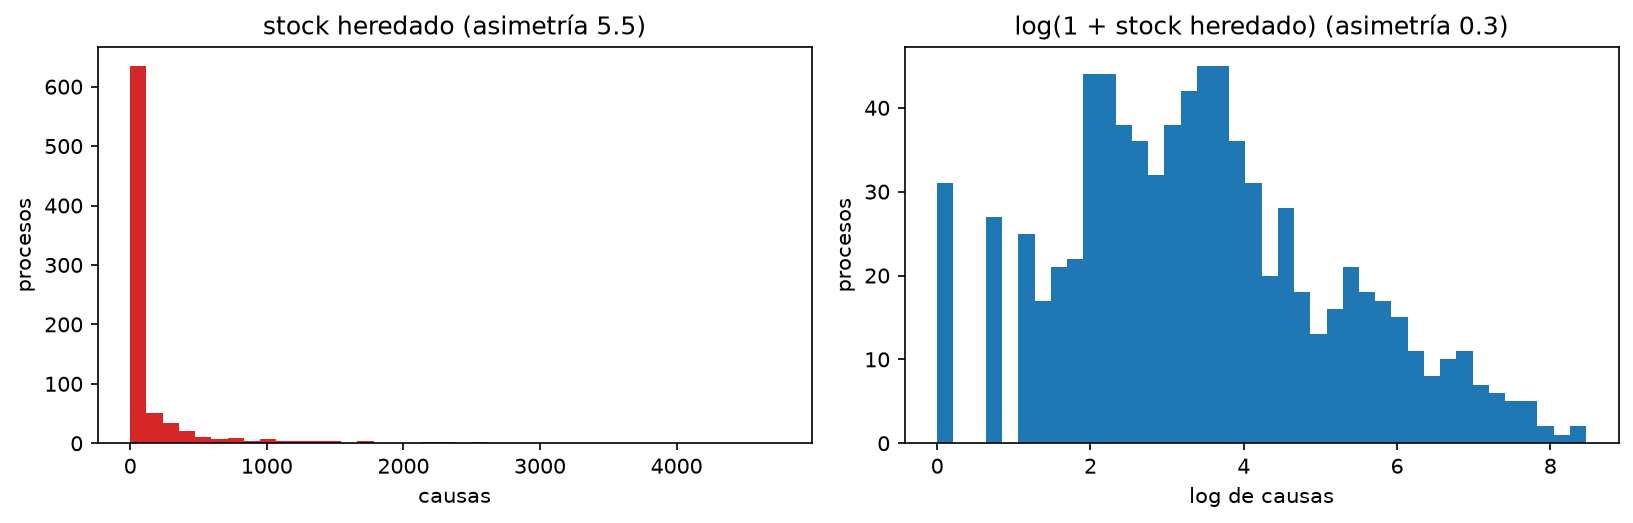
\includegraphics[width=0.85\linewidth]{nb19_3.png}
  \caption{El stock heredado tiene una cola larga; su logaritmo es casi simétrico. Notebook 19.}
  \label{fig:asimetria}
\end{figure}

\subsection{Conversión}

\begin{itemize}
  \item \textbf{Objetivo.} Días $\rightarrow \log(1+\text{días})$, con tope de 10 años. En logaritmo, equivocarse por el
  doble pesa lo mismo en un proceso de 30 días que en uno de 900.
  \item \textbf{Tipos.} Los conteos con vacíos de pandas (\texttt{Int64} con \texttt{<NA>}) pasan a \texttt{float64};
  las categorías, a texto.
  \item \textbf{Ingeniería de variables.} \nIngenieria{} variables calculadas fila por fila, sin promedios de grupo, para
  que el despliegue pueda recalcularlas con la misma fórmula: logaritmos, la presión del stock, los ingresos y el stock
  por juzgado, la proporción de puestos vacantes y de causas recibidas por excusa, y una marca de «sin stock heredado».
  \item \textbf{Historia.} \nHistoricas{} variable de la serie por materia: la tendencia de las resoluciones el año
  anterior (tabla~\ref{tab:variables}).
  \item \textbf{One-hot.} Materia, departamento y ámbito se convierten en columnas 0/1. Un código 1, 2, 3 inventaría un
  orden que no existe. Las \nCompleta{} variables quedan en 41 columnas numéricas.
  \item \textbf{Escala.} Para el SVM, la regresión lineal y el Stacking, cada columna se lleva a media 0 y desvío 1: el SVM
  mide distancias, y sin escala la remuneración (millones) taparía a todo lo demás.
  \item \textbf{Partición.} \nEntrenamiento{} procesos (80~\%) para entrenar y ajustar, \nPrueba{} (20~\%) guardados para
  la evaluación final, estratificada por quintiles del tiempo: las dos partes tienen la misma mezcla de procesos rápidos
  y lentos.
\end{itemize}

Todos los pasos (menos el del objetivo) viven dentro de un \texttt{Pipeline} de scikit-learn \cite{sklearn}: se ajustan
solo con los datos de entrenamiento de cada pliegue y se aplican igual a los datos de validación y de prueba.

\begin{table}[H]
  \centering\footnotesize
  \caption{Las \nCompleta{} variables del modelo: \nOriginales{} originales, \nIngenieria{} de ingeniería y
  \nHistoricas{} histórica, con su conversión y su correlación de Spearman con el objetivo (las categóricas no tienen).
  Notebook 19.}
  \label{tab:variables}
  \resizebox{\linewidth}{!}{\begin{tabular}{llllr}
\toprule
Variable & Descripción & Grupo & Conversión & $\rho$ Spearman \\
\midrule
\texttt{materia\_homologada} & materia & original & one-hot & --- \\
\texttt{ambito} & capital o provincia & original & one-hot & --- \\
\texttt{departamento\_derivado} & departamento & original & one-hot & --- \\
\texttt{pendientes\_inicio\_efectivo} & stock heredado & original & mediana & 0,04 \\
\texttt{nuevas\_ingresadas} & causas nuevas & original & mediana & 0,24 \\
\texttt{recibidas\_excusa\_recusacion} & recibidas por excusa & original & mediana & 0,07 \\
\texttt{preliminares\_formalizados} & preliminares formalizados & original & cero estructural + mediana & 0,10 \\
\texttt{cautelares\_formalizados} & cautelares formalizados & original & cero estructural + mediana & 0,05 \\
\texttt{ingresos\_totales} & ingresos del año & original & mediana & 0,24 \\
\texttt{atendidas} & causas atendidas & original & mediana & 0,17 \\
\texttt{num\_juzgados\_pagina} & juzgados (materia y territorio) & original & mediana & 0,08 \\
\texttt{recurso\_juzgados\_publicados} & juzgados del territorio & original & mediana & 0,04 \\
\texttt{recurso\_tribunales\_publicados} & tribunales del territorio & original & mediana & 0,08 \\
\texttt{recurso\_conciliadores\_publicados} & conciliadores del territorio & original & mediana & 0,05 \\
\texttt{personal\_items\_mujer} & puestos ocupados por mujeres & original & mediana & 0,07 \\
\texttt{personal\_items\_varon} & puestos ocupados por varones & original & mediana & 0,07 \\
\texttt{personal\_items\_acefalias} & puestos vacantes & original & mediana & 0,06 \\
\texttt{personal\_items\_total} & puestos totales & original & mediana & 0,06 \\
\texttt{personal\_remun\_total} & remuneración total & original & mediana & 0,06 \\
\texttt{log\_stock\_inicial} & log(1 + stock heredado) & ingeniería & mediana & 0,04 \\
\texttt{log\_ingresos} & log(1 + ingresos del año) & ingeniería & mediana & 0,24 \\
\texttt{presion\_stock} & stock heredado / (ingresos del año + 1) & ingeniería & mediana & -0,23 \\
\texttt{ingresos\_por\_juzgado} & ingresos del año / juzgados & ingeniería & mediana & 0,20 \\
\texttt{stock\_por\_juzgado} & stock heredado / juzgados & ingeniería & mediana & 0,01 \\
\texttt{prop\_acefalias} & puestos vacantes / puestos totales & ingeniería & mediana & -0,01 \\
\texttt{prop\_excusa} & recibidas por excusa / (ingresos del año + 1) & ingeniería & mediana & 0,08 \\
\texttt{sin\_stock\_inicial} & 1 si no había stock heredado & ingeniería & mediana & 0,05 \\
\bottomrule
\end{tabular}
}
\end{table}

%=====================================================================
\section{Modelo}

\paragraph{Protocolo.} Todos los modelos se entrenan y se comparan solo con el 80~\% de entrenamiento, usando
\textbf{validación cruzada de 5 pliegues}: el entrenamiento se parte en cinco, se entrena con cuatro y se mide con el
quinto, cinco veces. Como referencias se usan una \textbf{línea base} que siempre dice el tiempo promedio, la
\textbf{fórmula ingenua} (stock heredado entre ingresos por 365, sin aprender nada) y una \textbf{regresión lineal} con
freno a los pesos grandes (Ridge).

\begin{idea}[title={Cómo se mide el error}]
La métrica principal es el \textbf{error absoluto medio en $\log(1+\text{días})$} (MAE): es la que minimiza el ajuste de
hiperparámetros. Para leerla en palabras se reportan tres medidas más:
\begin{itemize}
  \item \textbf{dentro del doble:} de cada 100 procesos, en cuántos el tiempo real quedó entre la mitad y el doble de lo
  estimado;
  \item \textbf{factor mediano:} la mitad de las estimaciones se equivoca por menos que este factor ($\times1{,}5$ = hasta
  50~\% de más o de menos);
  \item \textbf{$R^2$ en log:} qué parte de las diferencias de tiempo entre procesos explica el modelo (0 = nada, 1 = todo).
\end{itemize}
\end{idea}

\subsection{SVM}
La máquina de vectores de soporte \cite{cortes1995}, en su versión de regresión (SVR), busca una curva que deje a la
mayoría de los procesos dentro de un \emph{tubo} de ancho $\varepsilon$ alrededor de ella: los errores menores que
$\varepsilon$ no se castigan, y los que quedan fuera, sí, en proporción a \texttt{C}. Con el \emph{kernel} RBF la curva
puede doblarse, y \texttt{gamma} decide qué tan lejos llega la influencia de cada punto. Necesita las variables escaladas.

\subsection{Bagging}
\emph{Bootstrap aggregating} \cite{breiman1996}: se entrenan muchos árboles de regresión, cada uno con una muestra con
reemplazo de las filas, y se \emph{promedian} sus estimaciones. Cada árbol solo es inestable; el promedio reduce esa
varianza. Se probaron dos versiones: un \texttt{BaggingRegressor} de árboles y el \textbf{Random Forest}
\cite{breiman2001}, que además hace que cada corte mire solo un subconjunto de variables al azar.

\subsection{Boosting}
Los árboles se entrenan \emph{en secuencia}, cada uno enfocado en lo que los anteriores hicieron mal. En
\textbf{AdaBoost} \cite{freund1997} cada árbol da más peso a los procesos que el anterior estimó peor. En
\textbf{Gradient Boosting} \cite{friedman2001} cada árbol se ajusta al error residual del conjunto anterior, y una tasa de
aprendizaje controla cuánto corrige cada uno.

\subsection{Stacking}
Combina modelos distintos \cite{wolpert1992}: el SVM, el Random Forest y el Gradient Boosting (con sus hiperparámetros
ajustados) producen una estimación cada uno, y una regresión lineal aprende cuánto confiar en cada uno. Para que esa
regresión no aprenda de estimaciones hechas sobre los mismos datos con que se entrenó cada modelo, usa predicciones
\emph{fuera de pliegue}.

\subsection{Hiperparámetros}
Un hiperparámetro es una perilla que se fija antes de entrenar (cuántos árboles, qué tan profundos, cuánto castigar los
errores) y que no se aprende de los datos: se elige probando combinaciones con la misma validación cruzada.

\begin{itemize}
  \item \textbf{SVM: búsqueda en grilla} (\texttt{GridSearchCV}) de 48 combinaciones (4 valores de \texttt{C}, 6 de
  \texttt{gamma} y 2 de \texttt{epsilon}). El error va de \maeSvmMax{} a \maeSvmMin; el mejor punto es
  \texttt{C}~$=$~\svmC, \texttt{gamma}~$=$~\svmGamma{} y \texttt{epsilon}~$=$~\svmEpsilon: una curva suave con un castigo
  moderado. Con \texttt{gamma} alto la curva se ondula demasiado y el modelo sobreajusta (figura~\ref{fig:grilla}).
  \item \textbf{Resto: búsqueda aleatoria} (\texttt{RandomizedSearchCV}) de 30 combinaciones. Con cuatro a seis perillas
  la grilla completa tendría cientos de combinaciones, y la búsqueda aleatoria llega a valores casi igual de buenos con
  mucho menos costo.
\end{itemize}

\begin{figure}[H]
  \centering
  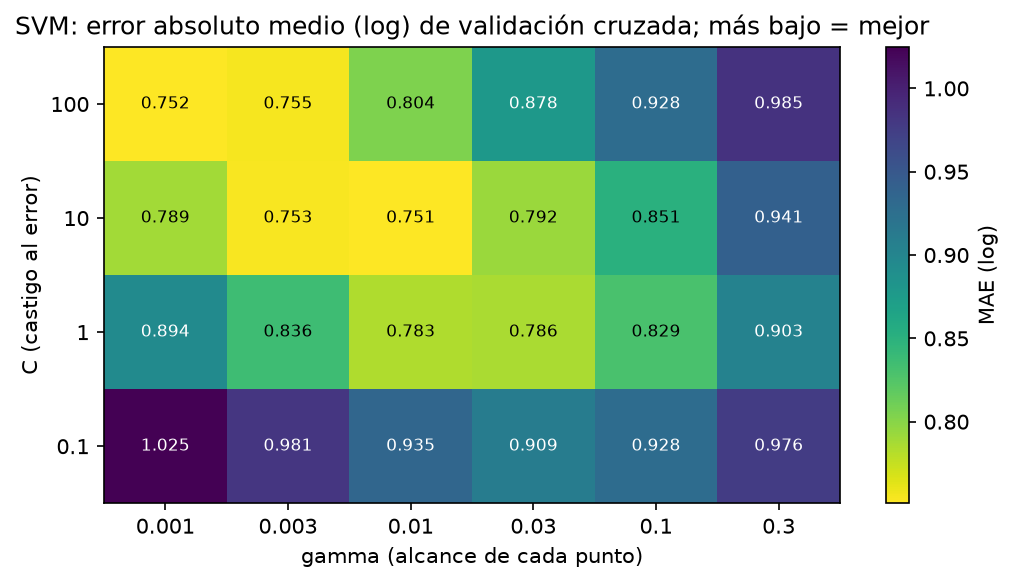
\includegraphics[width=0.72\linewidth]{nb20_2.png}
  \caption{Error de validación cruzada del SVM para cada par (\texttt{C}, \texttt{gamma}), con el mejor
  \texttt{epsilon}; más bajo es mejor. Notebook 20.}
  \label{fig:grilla}
\end{figure}

\begin{table}[H]
  \centering\small
  \caption{Hiperparámetros elegidos. Notebook 20.}
  \label{tab:hp}
  \begin{tabular}{lll}
\toprule
Modelo & Hiperparámetro & Valor elegido \\
\midrule
SVM & \texttt{C} & 10 \\
SVM & \texttt{epsilon} & 0,1 \\
SVM & \texttt{gamma} & 0,01 \\
Regresión lineal (Ridge) & \texttt{alpha} & 10 \\
Bagging & \texttt{n\_estimators} & 200 \\
Bagging & \texttt{max\_samples} & 0,5 \\
Bagging & \texttt{max\_features} & 1 \\
Bagging & \texttt{estimator\_\_min\_samples\_leaf} & 1 \\
Random Forest & \texttt{n\_estimators} & 400 \\
Random Forest & \texttt{min\_samples\_leaf} & 2 \\
Random Forest & \texttt{max\_features} & 0,5 \\
Random Forest & \texttt{max\_depth} & 8 \\
AdaBoost & \texttt{n\_estimators} & 100 \\
AdaBoost & \texttt{loss} & exponential \\
AdaBoost & \texttt{learning\_rate} & 0,05 \\
AdaBoost & \texttt{estimator\_\_max\_depth} & 6 \\
Gradient Boosting & \texttt{subsample} & 0,85 \\
Gradient Boosting & \texttt{n\_estimators} & 100 \\
Gradient Boosting & \texttt{min\_samples\_leaf} & 10 \\
Gradient Boosting & \texttt{max\_depth} & 4 \\
Gradient Boosting & \texttt{loss} & huber \\
Gradient Boosting & \texttt{learning\_rate} & 0,03 \\
\bottomrule
\end{tabular}

\end{table}

\paragraph{Resultados.} Todos los modelos entrenados superan a las dos referencias (tabla~\ref{tab:cv} y
figura~\ref{fig:ajuste}): la línea base tiene un error de \maeCvBase{} y la fórmula ingenua \maeCvIngenua; el mejor modelo,
\textbf{\mejorModelo}, baja a \mejorMaeCv. Seis modelos quedan juntos arriba (Stacking \maeCvStacking, Gradient Boosting
\maeCvGradientBoosting, SVM \maeCvSVM, Bagging \maeCvBagging, Random Forest \maeCvRandomForest, AdaBoost \maeCvAdaBoost): las
diferencias son menores que el desvío entre pliegues (alrededor de 0,08), así que con estos datos no se puede decir que
uno sea claramente mejor. La regresión lineal queda atrás (\maeCvRidge): parte de la relación entre carga y tiempo no es
una suma de efectos. Ajustar hiperparámetros ayuda a todos, sobre todo a AdaBoost (de \maeDefAdaBoost{} a
\maeCvAdaBoost) y a Bagging (de \maeDefBagging{} a \maeCvBagging). Gradient Boosting eligió la pérdida \emph{Huber}, que
trata los errores grandes como lineales: así unos pocos procesos extremos no arrastran a los demás.

\paragraph{La fórmula ingenua acierta seguido, pero falla por mucho.} Deja a casi 6 de cada 10 procesos dentro del doble,
pero explica casi nada de las diferencias entre procesos ($R^2$ cercano a 0), porque en los procesos con mucha fila se queda
muy corta. Los modelos explican alrededor del 40~\%.

\begin{table}[H]
  \centering\small
  \caption{Validación cruzada de 5 pliegues en el entrenamiento: error (MAE en log) con los valores por defecto y
  ajustado, desvío entre pliegues, proporción dentro del doble y $R^2$ del modelo ajustado. Notebook 20.}
  \label{tab:cv}
  \resizebox{\linewidth}{!}{\begin{tabular}{llrrrrr}
\toprule
Modelo & Familia & MAE por defecto & MAE ajustado & Desvío & Dentro del doble & $R^2$ \\
\midrule
Línea base (promedio) & referencia & 1,085 & 1,085 & 0,120 & 43\,\% & -0,016 \\
Fórmula ingenua & referencia & 0,888 & 0,888 & 0,044 & 58\,\% & 0,046 \\
Regresión lineal (Ridge) & referencia & 0,796 & 0,787 & 0,093 & 61\,\% & 0,384 \\
SVM & SVM & 0,790 & 0,751 & 0,092 & 64\,\% & 0,441 \\
Bagging & Bagging & 0,804 & 0,752 & 0,083 & 62\,\% & 0,429 \\
Random Forest & Bagging & 0,767 & 0,752 & 0,076 & 63\,\% & 0,430 \\
AdaBoost & Boosting & 0,890 & 0,755 & 0,067 & 63\,\% & 0,399 \\
Gradient Boosting & Boosting & 0,780 & 0,746 & 0,080 & 65\,\% & 0,438 \\
Stacking & Stacking & 0,751 & 0,738 & 0,088 & 64\,\% & 0,457 \\
\bottomrule
\end{tabular}
}
\end{table}

\begin{figure}[H]
  \centering
  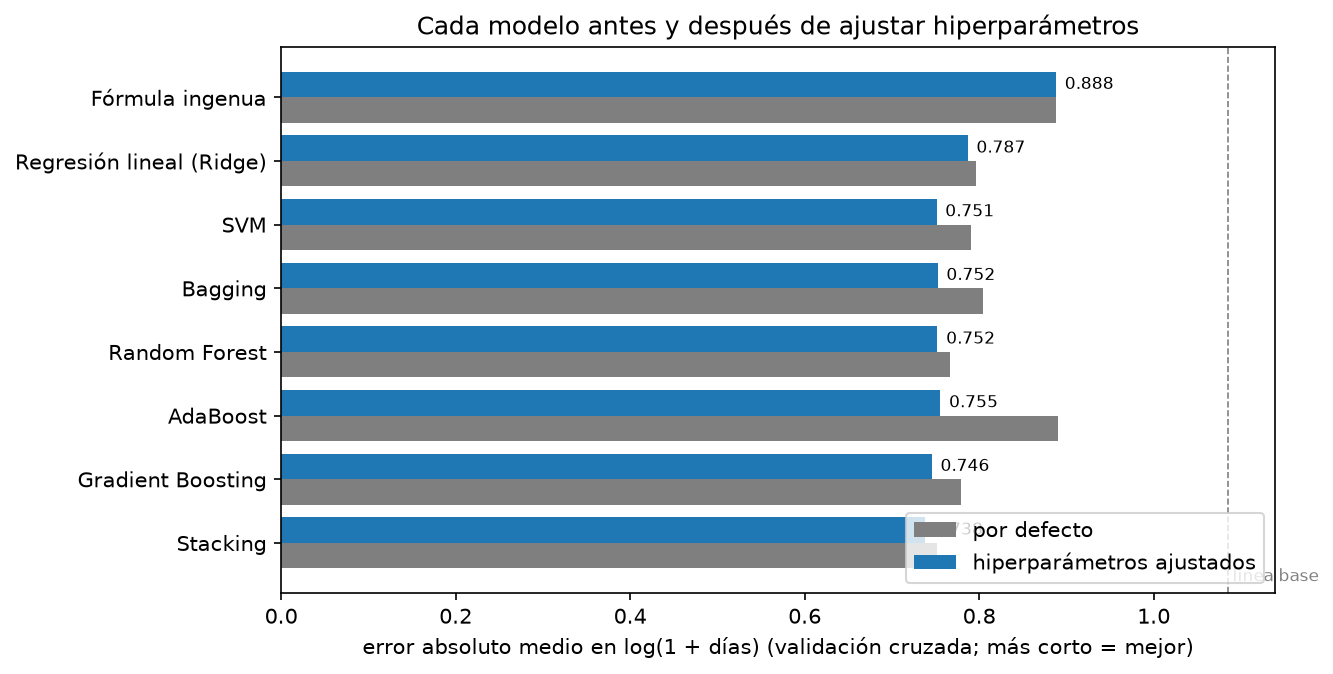
\includegraphics[width=0.85\linewidth]{nb20_1.png}
  \caption{Cada modelo antes y después de ajustar hiperparámetros (línea gris: la línea base). Notebook 20.}
  \label{fig:ajuste}
\end{figure}

%=====================================================================
\section{Evaluación}

\subsection{Métricas en la prueba}
Los \nPrueba{} procesos de prueba se usan por primera vez aquí (tabla~\ref{tab:test}). El mejor modelo de la validación,
\mejorModelo, obtiene un error de \mejorMaePrueba: deja al \textbf{\mejorDobPrueba~\%} de los procesos entre la mitad y el
doble de su tiempo real, la mitad de sus estimaciones se equivoca por menos de $\times$\mejorFactorPrueba{} y su error
mediano es de \mejorDiasPrueba{} días. Las referencias: línea base \maePruebaBase{} (\dobPruebaBase~\% dentro del doble) y
fórmula ingenua \maePruebaIngenua{} (\dobPruebaIngenua~\%, pero $R^2$ de \rdosPruebaIngenua). Con \nPrueba{} procesos,
diferencias de 0,02 entre modelos están dentro del ruido: en la prueba la regresión lineal (\maePruebaRidge) queda casi
igual que los ensambles.

\begin{table}[H]
  \centering\small
  \caption{Métricas en la prueba. Notebook 21.}
  \label{tab:test}
  \resizebox{\linewidth}{!}{\begin{tabular}{lrrrrr}
\toprule
Modelo & Exactitud & Precisión & Recall & F1 & ROC-AUC \\
\midrule
Línea base (clase mayoritaria) & 0,508 & 0,000 & 0,000 & 0,000 & 0,500 \\
Regresión logística & 0,657 & 0,643 & 0,680 & 0,661 & 0,716 \\
SVM & 0,661 & 0,648 & 0,680 & 0,664 & 0,735 \\
Bagging & 0,661 & 0,644 & 0,697 & 0,669 & 0,729 \\
Random Forest & 0,653 & 0,632 & 0,705 & 0,667 & 0,731 \\
AdaBoost & 0,629 & 0,603 & 0,721 & 0,657 & 0,700 \\
Gradient Boosting & 0,645 & 0,633 & 0,664 & 0,648 & 0,736 \\
Stacking & 0,661 & 0,646 & 0,689 & 0,667 & 0,741 \\
\bottomrule
\end{tabular}
}
\end{table}

\begin{figure}[H]
  \centering
  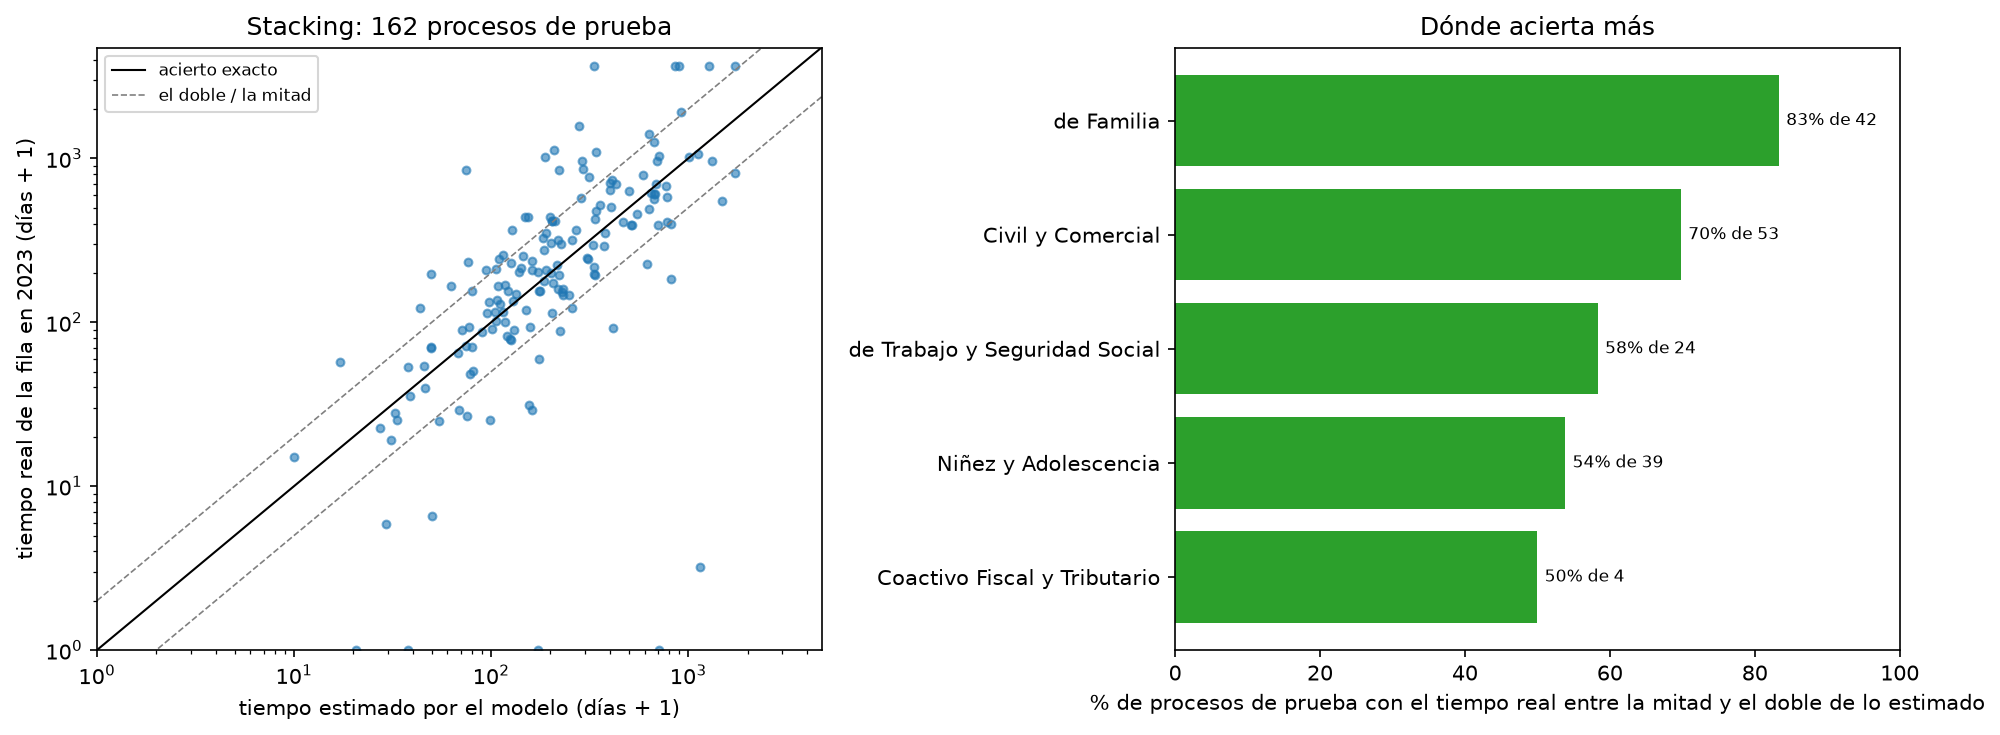
\includegraphics[width=\linewidth]{nb21_1.png}
  \caption{Izquierda: tiempo estimado por \mejorModelo{} contra el tiempo real de los procesos de prueba (escala
  logarítmica; las líneas punteadas marcan la mitad y el doble). Derecha: proporción dentro del doble por materia.
  Notebook 21.}
  \label{fig:prueba}
\end{figure}

\paragraph{Acierta mucho más en los procesos grandes.} Dentro del doble: \dobTamanoA~\% de los procesos con 10 a 30
causas, \dobTamanoB~\% con 31 a 100, \dobTamanoC~\% con 101 a 500 y \textbf{\dobTamanoD~\%} con más de 500
(tabla~\ref{tab:tamano}). En un proceso con miles de causas la fila es estable; en uno con 15, una sola causa cambia mucho
el tiempo. Por materia acierta más en familia y civil que en niñez y trabajo (figura~\ref{fig:prueba}).

\begin{table}[H]
  \centering\small
  \caption{Error de \mejorModelo{} en la prueba según el tamaño del proceso. Notebook 21.}
  \label{tab:tamano}
  \begin{tabular}{lrrr}
\toprule
Causas atendidas & Procesos de prueba & MAE (log) & Dentro del doble \\
\midrule
10-30 & 43 & 0,911 & 47\,\% \\
31-100 & 48 & 0,745 & 62\,\% \\
101-500 & 37 & 0,738 & 78\,\% \\
más de 500 & 34 & 0,300 & 88\,\% \\
\bottomrule
\end{tabular}

\end{table}

\subsection{Importancia de las variables}
Se midió por \textbf{permutación}: se barajan los valores de una variable entre las filas y se mide cuánto \emph{sube} el
error. Si sube mucho, el modelo dependía de ella. Sirve para cualquier modelo, incluido el SVM, que no tiene importancias
propias. Se calculó sobre \mejorModelo, en los pliegues de validación del entrenamiento (5 pliegues $\times$ 10 barajadas),
nunca en la prueba, para que elegir las variables no «espíe» los datos con que se evalúa. Como comparación se incluye la
importancia por impureza del Random Forest.

Lo que más usa el modelo es la \textbf{carga en relación con la capacidad}: \topVarA, \topVarB, \topVarC, \topVarD{} y
\topVarE{} (tabla~\ref{tab:imp} y figura~\ref{fig:imp}). Las cinco salen de solo tres datos: la fila que espera (stock
heredado), las causas que entran y los juzgados. El personal, las vacantes, la remuneración y el ámbito importan poco. La
variable histórica queda en el puesto \rangoHistorica{} (\impHistorica): el ritmo de la materia en todo el país casi no dice
nada del tiempo de un proceso concreto. La historia sirvió más para \emph{validar la medida} que como pista del modelo.

\begin{table}[H]
  \centering\small
  \caption{Las 12 variables más importantes: cuánto sube el error al barajarlas (media y desvío entre pliegues) e
  importancia por impureza del Random Forest. Notebook 21.}
  \label{tab:imp}
  \begin{tabular}{rllrrr}
\toprule
\# & Variable & Grupo & Permutación & Desvío & Impureza RF \\
\midrule
1 & log del stock heredado & ingeniería & 0,1549 & 0,0988 & 0,044 \\
2 & presión del stock & ingeniería & 0,1455 & 0,0773 & 0,367 \\
3 & log de los ingresos & ingeniería & 0,1233 & 0,0686 & 0,033 \\
4 & ingresos por juzgado & ingeniería & 0,0548 & 0,0135 & 0,072 \\
5 & stock por juzgado & ingeniería & 0,0264 & 0,0185 & 0,062 \\
6 & stock heredado & original & 0,0149 & 0,0153 & 0,047 \\
7 & departamento & original & 0,0137 & 0,0111 & 0,012 \\
8 & puestos ocupados por mujeres & original & 0,0105 & 0,0090 & 0,019 \\
9 & materia & original & 0,0095 & 0,0073 & 0,031 \\
10 & puestos vacantes & original & 0,0080 & 0,0042 & 0,033 \\
11 & puestos totales & original & 0,0074 & 0,0089 & 0,020 \\
12 & remuneración total & original & 0,0070 & 0,0070 & 0,024 \\
\bottomrule
\end{tabular}

\end{table}

\begin{figure}[H]
  \centering
  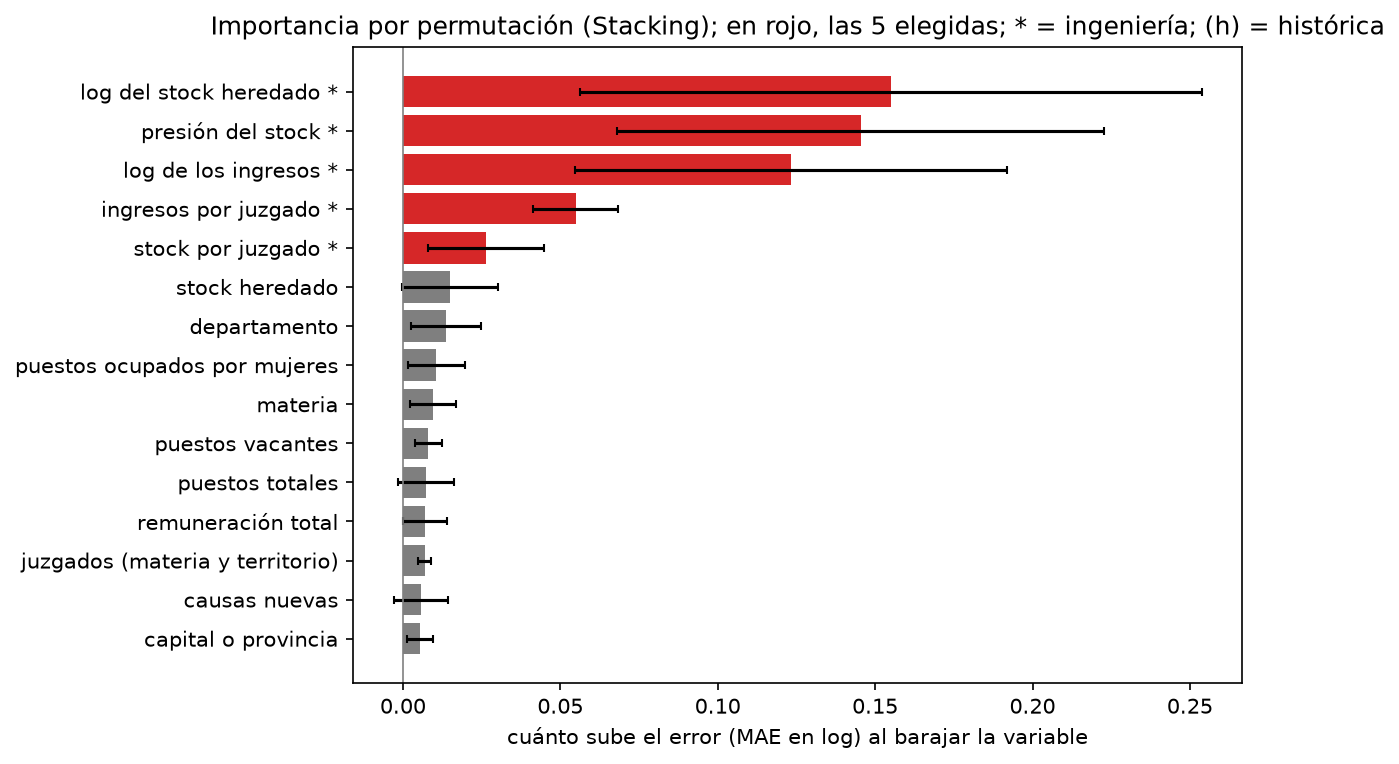
\includegraphics[width=0.8\linewidth]{nb21_3.png}
  \caption{Importancia por permutación; en rojo, las 5 elegidas; con asterisco, las de ingeniería; (h), la histórica.
  Notebook 21.}
  \label{fig:imp}
\end{figure}

\subsection{Tres versiones: \nOriginales, \nCompleta{} y 5 variables}
Cada modelo se volvió a entrenar con tres conjuntos de variables: las \nOriginales{} originales, las \nCompleta{} con
ingeniería e historia y las 5 más importantes (tabla~\ref{tab:versiones} y figura~\ref{fig:versiones}).

\begin{itemize}
  \item \textbf{Con ingeniería e historia (\nCompleta) es la mejor en todos los modelos.} \mejorModelo:
  \maeVVeintiochoCvStacking{} en validación y \maeVVeintiochoPruebaStacking{} en la prueba.
  \item \textbf{Las \nOriginales{} originales} pierden bastante (\mejorModelo{} \maeVDiecinueveCvStacking{} y
  \maeVDiecinuevePruebaStacking; la regresión lineal \maeVDiecinueveCvRidge): los cocientes y logaritmos que arma la
  ingeniería son buena parte de la señal, y los modelos lineales no los pueden construir solos.
  \item \textbf{Las 5 más importantes quedan cerca de las \nCompleta} (\mejorModelo: \maeVCincoCvStacking{} y
  \maeVCincoPruebaStacking; SVM: \maeVCincoCvSVM{} y \maeVCincoPruebaSVM). El modelo pequeño casi no pierde, porque esas
  cinco ya concentran la carga y la capacidad.
\end{itemize}

\begin{table}[H]
  \centering\small
  \caption{Error (MAE en log) de cada modelo con cada versión de las variables, en validación cruzada (CV) y en la
  prueba. Notebook 21.}
  \label{tab:versiones}
  \begin{tabular}{lrrrrrr}
\toprule
Modelo & 19 (CV) & 19 (prueba) & 27 (CV) & 27 (prueba) & 5 (CV) & 5 (prueba) \\
\midrule
Regresión logística & 0,584 & 0,604 & 0,730 & 0,716 & 0,659 & 0,619 \\
SVM & 0,595 & 0,639 & 0,729 & 0,735 & 0,649 & 0,631 \\
Bagging & 0,735 & 0,712 & 0,753 & 0,729 & 0,704 & 0,658 \\
Random Forest & 0,739 & 0,715 & 0,753 & 0,731 & 0,705 & 0,662 \\
AdaBoost & 0,709 & 0,704 & 0,728 & 0,700 & 0,714 & 0,660 \\
Gradient Boosting & 0,732 & 0,739 & 0,744 & 0,736 & 0,712 & 0,663 \\
Stacking & 0,737 & 0,718 & 0,753 & 0,741 & 0,705 & 0,664 \\
\bottomrule
\end{tabular}

\end{table}

\begin{figure}[H]
  \centering
  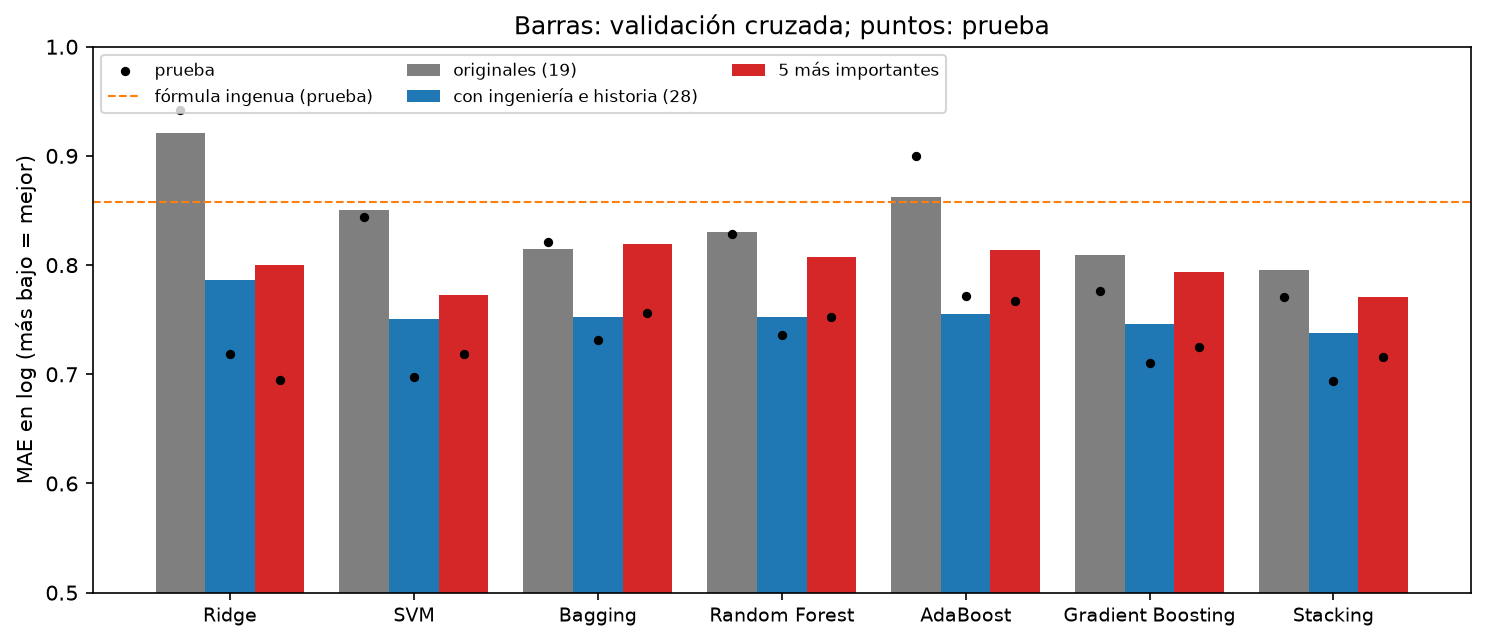
\includegraphics[width=0.9\linewidth]{nb21_4.png}
  \caption{Barras: validación cruzada; puntos: prueba; línea naranja: la fórmula ingenua en la prueba. Más bajo es mejor.
  Notebook 21.}
  \label{fig:versiones}
\end{figure}

\subsection{Control de robustez}
El mismo tipo de proceso (por ejemplo, «divorcio») aparece en varios departamentos. Si el modelo solo «recordara» cada
tipo, le iría bien en la validación normal y mal con un tipo nuevo. Con validación por grupos (\texttt{GroupKFold}), todas
las filas de un tipo de proceso quedan del mismo lado. \mejorModelo{} con \nCompleta{} variables sube de
\maeVVeintiochoCvStacking{} a \maeGruposVeintiochoStacking{} (+\difGruposVeintiochoStacking) y con 5 variables apenas
+\difGruposCincoStacking: el modelo generaliza a tipos de proceso que no vio. El SVM con \nCompleta{} variables es el que
más pierde (tabla~\ref{tab:robustez}).

\begin{table}[H]
  \centering\small
  \caption{Validación cruzada normal y por grupos de tipo de proceso (MAE en log). Notebook 21.}
  \label{tab:robustez}
  \begin{tabular}{llrrr}
\toprule
Versión & Modelo & MAE CV normal & MAE por grupos & Diferencia \\
\midrule
originales (19) & Stacking & 0,796 & 0,810 & 0,014 \\
originales (19) & Random Forest & 0,830 & 0,822 & -0,008 \\
originales (19) & SVM & 0,850 & 0,875 & 0,025 \\
con ingeniería e historia (28) & Stacking & 0,738 & 0,764 & 0,026 \\
con ingeniería e historia (28) & Random Forest & 0,752 & 0,766 & 0,014 \\
con ingeniería e historia (28) & SVM & 0,751 & 0,812 & 0,061 \\
5 más importantes & Stacking & 0,770 & 0,778 & 0,007 \\
5 más importantes & Random Forest & 0,807 & 0,831 & 0,024 \\
5 más importantes & SVM & 0,773 & 0,771 & -0,002 \\
\bottomrule
\end{tabular}

\end{table}

%=====================================================================
\section{Despliegue}

Un modelo solo sirve si alguien lo puede usar. El modelo de 5 variables se publicó como una \textbf{página web pública}
en \url{https://proyanalisis.maxi42.space/}: la persona elige materia, tipo de proceso y lugar, y ve cuánto tardaría un
caso como el suyo. La web de documentación del proyecto tiene además una versión de clase
(\texttt{web/prediccion.html}) donde se escriben los tres datos a mano.

\subsection{El modelo exportado}

\paragraph{Qué modelo.} Entre los modelos de árboles, que se pueden exportar a un archivo de datos, el de menor error de
validación cruzada con 5 variables fue \textbf{\modeloDesplegado} (\maeVCincoCvGradientBoosting; Random Forest
\maeVCincoCvRandomForest, Bagging \maeVCincoCvBagging). Stacking y SVM quedaron apenas mejor, pero no se pueden pasar a un
archivo de árboles. Tiene \nArboles{} árboles y se entrena con el mismo 80~\% de entrenamiento, de modo que las métricas de
la prueba son las del modelo publicado.

\paragraph{Qué pide.} Solo \nEntradas{} datos: la fila que espera (stock heredado), las causas que entran por año y los
juzgados. Las 5 variables se calculan en la página con las mismas fórmulas del notebook.

\paragraph{Qué tan bien estima.} En la prueba: error \maeDesplegado, \textbf{\dobDesplegado~\%} de los procesos dentro del
doble, factor mediano $\times$\factorDesplegado{} y error mediano de \diasDesplegado{} días. El mismo modelo con las
\nCompleta{} variables daba \maeDesplegadoVeintiocho: simplificar a 5 cuesta muy poco.

\paragraph{Cómo funciona.} Un árbol es una lista de preguntas «¿variable $\le$ umbral?» y un valor en cada hoja. El
notebook 22 copia esas preguntas y las hojas, junto con el preprocesamiento, a un archivo JSON de \pesoJson~MB. La página
lo lee, recorre los árboles en JavaScript, suma sus aportes ---el resultado es $\log(1+\text{días})$--- y lo pasa a días.
Una reimplementación en Python que lee \emph{solo} el JSON da la misma estimación que scikit-learn en los \nPrueba{}
procesos de prueba, con una diferencia máxima de $\difJson$.

\subsection{El rango probable}
Una sola cifra engaña: el modelo se equivoca, y más en los procesos chicos. Por eso cada estimación va con un
\textbf{rango}. Con validación cruzada se midió cuánto se equivocó el modelo en procesos que no había visto y se guardó
entre qué errores cayó la mitad central (del 25~\% al 75~\%), por separado según el tamaño del proceso
(tabla~\ref{tab:bandas}). En un proceso de 10 a 30 causas el rango va de $\times$\rangoChicoDesde{} a
$\times$\rangoChicoHasta{} de la estimación; en uno de más de 500, de $\times$\rangoGrandeDesde{} a
$\times$\rangoGrandeHasta. En la prueba, que no participó en el cálculo, cayó dentro de su rango el \coberturaRango~\% de
los procesos, cerca del 50~\% buscado.

\begin{table}[H]
  \centering\small
  \caption{El rango probable según el tamaño del proceso: la estimación se multiplica por estos factores. Notebook 22.}
  \label{tab:bandas}
  \begin{tabular}{lrrrr}
\toprule
Tamaño del proceso & Procesos (entren.) & Rango: $\times$ desde & $\times$ hasta & Dentro en la prueba \\
\midrule
10 a 30 causas & 163 & 0,43 & 2,35 & 25 de 43 \\
31 a 100 causas & 197 & 0,59 & 1,80 & 24 de 48 \\
101 a 500 causas & 177 & 0,70 & 1,56 & 19 de 37 \\
más de 500 causas & 109 & 0,66 & 1,44 & 24 de 34 \\
\bottomrule
\end{tabular}

\end{table}

\subsection{La página pública}

El notebook 23 arma el escenario de un \textbf{caso que entra al empezar 2024}: la fila que espera es lo que quedó
pendiente al cierre de 2023, los juzgados son los mismos y, como los ingresos de 2024 no se conocen, se usan los de 2023.
Con eso calcula la estimación de los 1.240 procesos con movimiento y escribe un JSON de 55~KB con nombres legibles
(«Familia», «El Alto», «Provincias de La Paz»). En los procesos con tiempo medido en 2023, la estimación para 2024 se
parece a lo medido: el 76~\% queda entre la mitad y el doble, y el 93~\% en los procesos con más de 500 causas, en línea con
lo que mostró la historia (de un año al siguiente el tiempo cambia poco). Para cada consulta la página muestra:

\begin{itemize}
  \item \textbf{«Si tu caso entra ahora, tardaría…»}: la estimación en palabras (días, meses o años), el rango probable
  y una regla que dibuja el rango, la estimación y lo que tardaba en 2023. Por ejemplo, para la asistencia familiar en
  Santa Cruz, el trámite con más causas del país, unos 12 meses (entre 8 y 17); para un divorcio en Sucre, unos 67 días
  (entre 44 y 97).
  \item \textbf{Lo que tardaba en 2023}, medido sin modelo, y \textbf{el ritmo de su materia}: las resueltas de 2020 a
  2023 en su ámbito.
  \item \textbf{El mismo trámite en otros lugares}, ordenado de más rápido a más lento.
  \item \textbf{La historia}: un gráfico del tiempo del país, las capitales y las provincias de 2007 a 2023 con lo que la
  fila de verdad tardó en vaciarse, y las dos comprobaciones de la sección 1.2.
  \item \textbf{Dónde un caso nuevo tardaría más}, una tabla para quien gestiona juzgados, filtrable por departamento y
  materia.
  \item Una advertencia en los procesos con menos de 10 causas, cuya estimación se apoya en procesos parecidos y es
  menos firme.
\end{itemize}

\noindent Al abrirse, la página recalcula las 1.240 estimaciones con los árboles del JSON y las compara con las de
Python: coinciden todas (sello «1.240 / 1.240 coinciden» en los detalles técnicos).

\subsection{Publicación en un VPS con Docker Compose}

Como el modelo corre en el navegador, el servidor no necesita Python ni scikit-learn: solo entrega archivos estáticos. Eso
hace al despliegue simple, barato y seguro: el servidor no recibe ni guarda lo que se consulta. La carpeta
\path{despliegue/} es independiente del resto del proyecto y tiene tres archivos de configuración
(tabla~\ref{tab:despliegue}).

\begin{table}[H]
  \centering\small
  \caption{Archivos del despliegue (carpeta \texttt{despliegue/}).}
  \label{tab:despliegue}
  \begin{tabular}{lp{11cm}}
    \toprule
    Archivo & Qué hace \\
    \midrule
    \texttt{Dockerfile} & Parte de la imagen \texttt{nginxinc/nginx-unprivileged:1.27-alpine} (el servidor web nginx
      corriendo como usuario sin privilegios), copia la configuración y la carpeta \texttt{sitio/}, expone el puerto 8080
      y define un chequeo de salud. \\
    \texttt{nginx.conf} & Sirve los archivos, comprime los JSON (gzip), envía cabeceras de seguridad (una política de
      contenido que solo permite archivos propios y las fuentes tipográficas), oculta la versión de nginx y responde
      \texttt{ok} en \texttt{/salud}. \\
    \texttt{docker-compose.yml} & Define el servicio: construye la imagen, publica el puerto 8080, reinicia el contenedor
      si se cae, lo deja de solo lectura, sin capacidades de Linux ni escalada de privilegios, y revisa \texttt{/salud}
      cada 30 segundos. \\
    \bottomrule
  \end{tabular}
\end{table}

\noindent El VPS usa \textbf{Dokploy}, un panel que despliega aplicaciones de Docker Compose desde un repositorio de
GitHub: lee \path{despliegue/docker-compose.yml} de la rama \texttt{main}, construye la imagen y la levanta. Su proxy
(Traefik) atiende el dominio \texttt{proyanalisis.maxi42.space}, obtiene el certificado HTTPS de Let's Encrypt y reenvía
las visitas al puerto 8080 del contenedor. Para actualizar el modelo se vuelven a ejecutar los notebooks 22 y 23 y se hace
\texttt{git push}: Dokploy vuelve a publicar. Sin Dokploy, en cualquier VPS con Docker basta:

\begin{verbatim}
cd despliegue && docker compose up -d --build
curl http://localhost:8080/salud          # responde: ok
\end{verbatim}

%=====================================================================
\section*{Conclusiones}
\addcontentsline{toc}{section}{Conclusiones}

\begin{enumerate}
  \item \textbf{Sí se puede estimar cuánto va a tardar un caso, con un rango.} Para el grupo de su tipo de proceso y
  lugar, el modelo deja a 2 de cada 3 procesos que no vio entre la mitad y el doble de su tiempo real, y a casi 9 de cada
  10 en los procesos grandes. No es un plazo legal, pero es mucho más de lo que hoy tiene quien inicia un proceso.
  \item \textbf{La historia respalda la medida.} En 17 años de datos, el tiempo estimado quedó a una mediana de
  \histErrVaciado~\% de lo que la fila de verdad tardó en vaciarse, y de un año al siguiente cambia una mediana de
  \histErrAnterior~\%. Por eso el último Anuario sirve para quien presenta su caso después, salvo en años excepcionales
  como la pandemia.
  \item \textbf{El tiempo depende de la carga relativa a la capacidad.} Lo que más explica cuánto se tarda es la fila
  heredada en relación con lo que entra y con los juzgados que la atienden; no las cantidades sueltas, ni el personal,
  ni ser capital o provincia. Tres datos bastan para el modelo publicado.
  \item \textbf{El preprocesamiento importa más que el modelo.} Entre los seis mejores modelos hay a lo sumo 0,02 de
  diferencia; entre trabajar con o sin las variables de ingeniería, entre 0,06 y 0,11 en los ensambles y 0,13 en la regresión
  lineal. Los ensambles ganan por poco, y el Stacking no supera con claridad a sus componentes.
  \item \textbf{La página lo pone al alcance de cualquiera.} Funciona en el navegador, reproduce exactamente al modelo de
  Python y se publica con Docker Compose en un VPS, sin código Python en el servidor.
\end{enumerate}

\section*{Limitaciones}
\addcontentsline{toc}{section}{Limitaciones}
\begin{itemize}
  \item \textbf{Es el tiempo de la fila, no el de un expediente.} El Anuario no sigue causas: el tiempo es el promedio de
  un grupo y supone que las causas salen en orden. Un caso concreto puede ir más rápido o más lento según el juzgado, las
  partes y lo que se pida.
  \item \textbf{El detalle por tipo de proceso es de un solo año.} La historia valida la medida para el país, las capitales
  y las provincias, no para cada tipo de proceso. Para saber cuánto acierta la estimación de 2024 en cada proceso hace
  falta un segundo Anuario con el mismo detalle. Los datos son de 2023: el Anuario más reciente con este detalle.
  \item \textbf{Los procesos chicos son poco firmes.} Con menos de 30 causas, el rango es amplio (de casi la mitad a más del
  doble).
  \item \textbf{Solo materias no penales,} porque las penales no publican resueltas.
  \item \textbf{Mide celeridad, no calidad} de las decisiones judiciales.
\end{itemize}

%=====================================================================
\begin{thebibliography}{9}
\bibitem{anuario} Consejo de la Magistratura de Bolivia. \emph{Anuario Estadístico Judicial 2023}. Jefatura Nacional de
  Estudios Técnicos y Estadísticos, 2024.
\bibitem{breiman1996} L.~Breiman. Bagging predictors. \emph{Machine Learning}, 24(2):123--140, 1996.
\bibitem{breiman2001} L.~Breiman. Random forests. \emph{Machine Learning}, 45(1):5--32, 2001.
\bibitem{cortes1995} C.~Cortes y V.~Vapnik. Support-vector networks. \emph{Machine Learning}, 20(3):273--297, 1995.
\bibitem{freund1997} Y.~Freund y R.~E.~Schapire. A decision-theoretic generalization of on-line learning and an
  application to boosting. \emph{Journal of Computer and System Sciences}, 55(1):119--139, 1997.
\bibitem{friedman2001} J.~H.~Friedman. Greedy function approximation: a gradient boosting machine. \emph{The Annals of
  Statistics}, 29(5):1189--1232, 2001.
\bibitem{wolpert1992} D.~H.~Wolpert. Stacked generalization. \emph{Neural Networks}, 5(2):241--259, 1992.
\bibitem{sklearn} F.~Pedregosa et al. Scikit-learn: machine learning in Python. \emph{Journal of Machine Learning
  Research}, 12:2825--2830, 2011.
\end{thebibliography}

%=====================================================================
\appendix
\section{Reproducción}

Los notebooks 19 a 23 leen la tabla curada \path{data/curated/features/dataset_analitico_curado.parquet} y las tablas del
capítulo 9 (\path{data/processed/}), que ya están en el repositorio: no hace falta el PDF. Desde la raíz del proyecto (en
Windows, \path{.venv\Scripts\pip}):

\begin{verbatim}
python -m venv .venv
.venv/bin/pip install -r requirements.txt

cd notebooks
for n in 19_preparacion_modelo 20_modelos 21_evaluacion \
         22_despliegue 23_sitio_publico; do
  jupyter nbconvert --to notebook --execute --inplace $n.ipynb
done

cd ../informe
pdflatex --disable-installer informe.tex     # dos veces
cd ../despliegue
docker compose up -d --build                 # abrir http://localhost:8080
# sin Docker: cd despliegue/sitio && python -m http.server 8000
\end{verbatim}

\noindent El notebook 22 escribe las tablas y las cifras de este informe en \path{informe/tablas/}, de modo que al
volver a correr el pipeline el informe se actualiza al compilar. Todas las salidas intermedias quedan en
\texttt{data/curated/modelo/}: la serie histórica y sus comprobaciones (\texttt{historia\_*.csv}), el diccionario de
variables, la partición, las métricas, los hiperparámetros, la importancia, las versiones y las bandas del rango. La
semilla es fija (42), así que cada ejecución da los mismos números.

\end{document}
